8. \begin{figure}[ht!]
\center{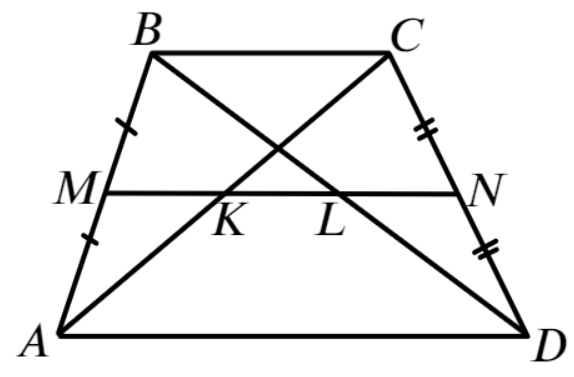
\includegraphics[scale=0.35]{g8-8.png}}
\end{figure}\\
Так как отрезок $MN$ является средней линией трапеции, он параллелен основаниям и проходит через середины $AB$ и $CD,$ а поэтому также содержит средние линии треугольников $ABC$ и $ACD,$ обозначим их $MK$ и $KN.$ Так как $MK+KN=8$см и $KN-MK=2$см, найдём $KN=5$см и $MK=3$см. Тогда $BC=2MK=6$см и $AD=2KN=10$см.\\
